\selectlanguage{english}
\clearpage
\section{Tool Evaluation and Framework Selection}

This chapter presents an evaluation of available tools and test frameworks that could be used to support the integration testing of IPC middleware. The goal is to identify solutions that align with the defined testing requirements and environmental constraints presented in the previous chapter. Based on a set of defined selection criteria, several tool candidates are reviewed and assessed in terms of their compatibility with eCAL and the specific demands of testing distributed communication systems.

\subsection{Selection Criteria}

To choose suitable testing tools and frameworks, several criteria were defined:

\begin{itemize}
	\item \textbf{Language Support:} The framework should support the languages already in use in the development environment, particularly C++, Python, and Bash.
	\item \textbf{Automation Capabilities:} Support for test automation, headless execution, and integration into CI/CD systems is essential.
	\item \textbf{Support for IPC Mechanisms:} Tools should be able to handle the orchestration of multi-process communication patterns, such as publish-subscribe and request-response.
	\item \textbf{Platform Compatibility:} The framework must work on Linux (especially Ubuntu 22.04), as this is the primary target platform.
	\item \textbf{Observability and Reporting:} Tools should offer logging, result exporting, or structured test result visualization (e.g., HTML reports).
\end{itemize}

\subsection{Evaluation of Tool Candidates}

Figure~\ref{fig:mm_orchestration} presents an overview of evaluated tools and orchestration options in the form of a mind map.

\begin{figure}[H]
	\centering
	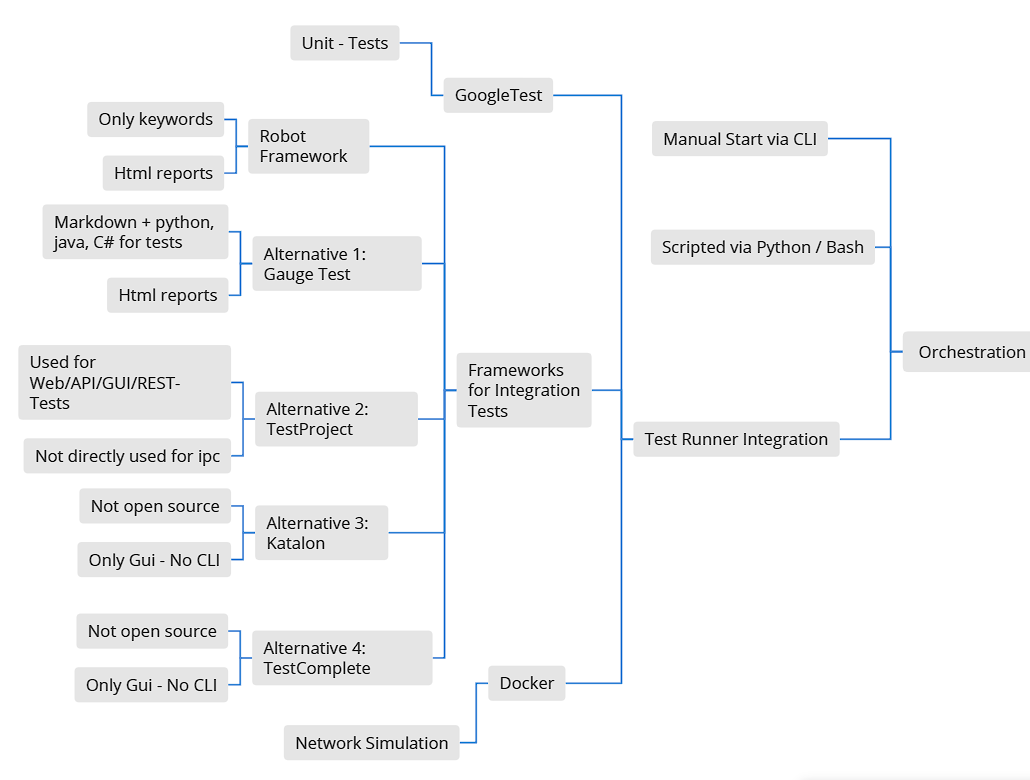
\includegraphics[width=\textwidth]{Images/mm_04_orchestration.png}
	\caption{Evaluation of orchestration and framework options for IPC testing}
	\label{fig:mm_orchestration}
\end{figure}

\subsubsection*{GoogleTest}

GoogleTest is a widely used unit testing framework for C++. It is already integrated into the eCAL source tree for verifying internal logic and module-level behavior. However, GoogleTest is primarily suited for unit testing and does not natively support multi-process orchestration. While it can be extended for IPC tests using wrappers or mocks, it lacks built-in support for orchestrating multiple processes across systems.

\subsubsection*{Robot Framework}

Robot Framework is a generic test automation framework that supports keyword-driven testing. It can be used with Python and Bash and is well-suited for automating high-level integration tests, including orchestration and output validation. With extensions like the \texttt{Process} and \texttt{OperatingSystem} libraries, Robot Framework can start and stop eCAL processes, validate log output, and perform assertions on results. HTML reports and logs are automatically generated, making it ideal for integration into CI pipelines.

\subsubsection*{Gauge Test}

Gauge is a test framework that supports writing specifications in Markdown and connecting them to test code written in Python, Java, or other languages. While it supports HTML reporting and automation, its community and ecosystem are smaller. It is also less commonly used for IPC scenarios.

\subsubsection*{TestProject, Katalon, and TestComplete}

These tools are designed for GUI, API, and web testing and are not suitable for low-level IPC testing. Most of them are not open source and depend on graphical interfaces, which makes them unsuitable for CLI-based test automation in eCAL.

\subsection{Feasibility for eCAL Integration}

Based on the evaluation, Robot Framework was selected as the most suitable tool for testing eCAL-based IPC systems. It fulfills the necessary automation and scripting requirements, supports orchestration of multiple processes, and provides structured reporting. Furthermore, it can be easily integrated with Docker for simulating multi-host scenarios and is compatible with Ubuntu-based environments. GoogleTest will continue to be used for unit-level testing inside the eCAL source code, while Robot Framework will handle higher-level integration tests.
